\documentclass{article}
\usepackage{amssymb}
\usepackage{amsmath}
\usepackage{bm}
\usepackage{cancel}
\usepackage{graphicx}
\author{Mann, J}
\title{Day 4 Notes}
\date{September 8, 2015}
\begin{document}
\maketitle{}
\renewcommand{\d}[0]{\mathrm{d}}
\newcommand{\dOne}[2]{\frac{\partial #1}{\partial #2}}
\newcommand{\dtwo}[2]{\frac{\partial^2 #1}{\partial #2^2}}
\newcommand{\diag}[1]{\bcancel{#1}}
\newcommand{\matr}[1]{\bm{#1}}
\begin{section}{Main}
  Notice: The thermodynamics I have developed using the Hansen or Cahn approach is general: liquid/vapor; liquid/liquid; liquid/solid; solid/solid interfaces are included in defining the excess quantities.

  The gibbs surface and surface of tension conepts require more work
  \begin{itemize}
    \item Recall the gibbs surface
    \item I will develop the surface of tension
    \item The Laplace equation when the surface is curved.
  \end{itemize}
\end{section}

\begin{section}
  {Gibbs surface}
  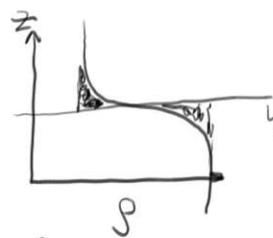
\includegraphics[height=100pt]{Day4NotesPics/gibbsSurface}
  \underline{Equimolar} surface Location.
  \begin{itemize}
    \item Comes from $\Gamma_1 = \int_{-\infty}^{+\infty}(\rho(z)-\rho^\pm)dz$
    \item  Now Deal with pressure:

    $\gamma^{def} = - \int_{-\infty}^{+\infty} (P_{11} - P_n) d z$
    \begin{itemize}
      \item $P_{11}$ is the pressure component parallel to the surface
      \item $P_n$ is the pressure component normal to the surface
    \end{itemize}

    This is the Gibbs surface definition of $\gamma$

    \item  The pressure tensor is a rank 2 tensor which means that the pressure can be thought of in terms of a matrix 
      $\matr{P} = \begin{pmatrix}
	P_{11} & P_{12} & P_{13} \\
	P_{21} & P_{22} & P_{23} \\
	P_{31} & P_{32} & P_{33} 
    \end{pmatrix}$
  \item $\matr{P} = \matr{P}^T$ (The pressure tensor is symmetric)
  \item $\matr{P} \equiv - \matr{\sigma}$
    (The pressure tensor is by definition the negative of the stress tensor)
    \item As soon as you say that the system could be anisotropic, a scalar Pressure is not valid.
    $\vec{F} = \hat{n}\cdot \sigma$
    $F_j = n_i \sigma_{ij}$
    $\vec{P}_j = - n_i \sigma_{ij}$
    $P^{ij} = P^{ji}?$ Most of the time.
  \end{itemize}
\end{section}
\begin{section}{Properties of P}
  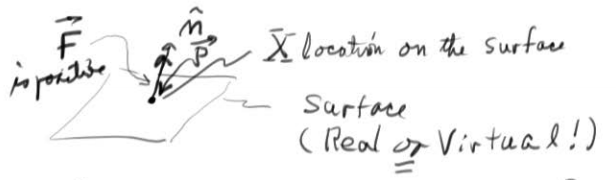
\includegraphics[height=100pt]{Day4NotesPics/Fdef}
  \begin{itemize}
    \item  $\vec{F} = \hat{n} \cdot \matr{\sigma}$ (Vector $\cdot$ Rank-2 gives a vector!)
    \item  $F_j = n_i \sigma_{ij}$ in component form.
    \item  $\vec{P} = -n_i \sigma_{ij}$ 
    \item  $n_i\sigma_{ij} = \sum\limits_{i=1}^3 n_i\sigma_{ij}$
    \item  $P_{ij} = P_{ji}$? Yes. This is symmetric.
    \item  $P_{ij} \in \mathbb{R}$? Yes.
    \item  $\hat{e}_j\vec{P}_i = -n_i\sigma_{ij}e_j = -e_j e_{ij} n_i$ (Where $\hat{e}_j$ is a direction in 3-space.  Note that $\hat{e}\cdot \matr{P} \cdot \hat{n}$ is a scalar Pressure.)
  \end{itemize}
\end{section}

\begin{section}{Test for isotropy}
  Does there exist a coordinate transformation (i.e. a 3x3 matrix $\matr{T}$ and its inverse $\matr{T}^{-1}$  such that 
  $\matr{T}^{-1} \matr{P} \matr{T} = 
  \begin{pmatrix}\vec{P}_{11} & 0 & 0 \\
  0 & \vec{P}_{22} &  0
  \\0 &  0 & \vec{P}_{33}
  \end{pmatrix}$ 
  If you can diagonlaize the pressure tensor, so long as $P_{ij} = P_{ji}$ and $P_{ij}$ are the real numbers, $\matr{T}$ exists!
\end{section}

\begin{section}{Isotropic Effects}
  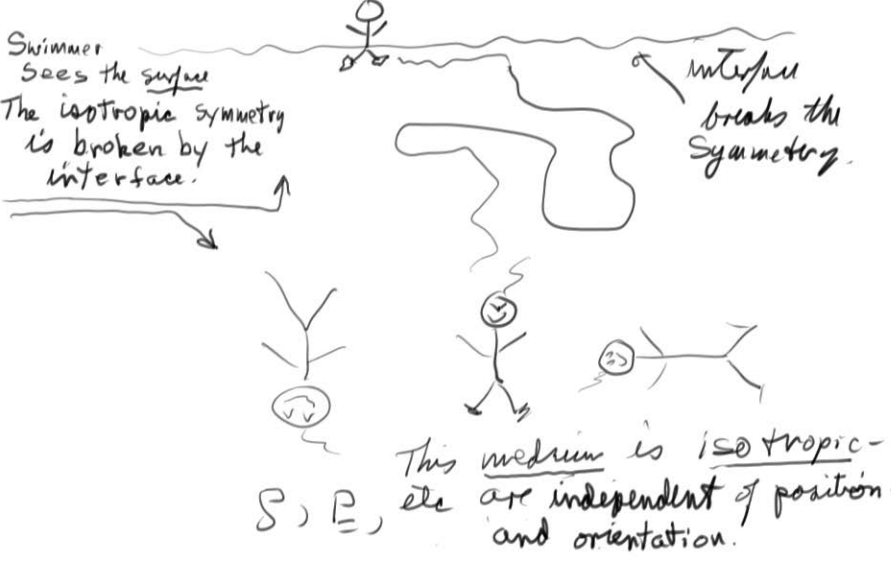
\includegraphics[height=200px]{Day4NotesPics/swimmer}
  \begin{itemize}
    \item Things like $\rho$, $\matr{P}$ are independent of the observer orientation.
    \item Interfaces fundamentally break the symmetry of systems.
    \item Think of a swimmer at midnight when it's cloudy. Underwater, there is no sense of direction. When the swimmer breaks the surface, however, the symmetry is broken, and the swimmer knows which direction is up.
  \end{itemize}

  \begin{itemize}
    \item There exists $\matr{T}, \matr{T}\matr{T}^{-1} = \matr{I}$ such that $\matr{T}^{-1}\matr{P}\matr{T} = \diag{\matr{P}} = \begin{pmatrix}
	\bar{P}_{11} & 0            & 0 \\
	0 & \bar{P}_{22} &  0\\
	0 &  0           & \bar{P}_{n}
      \end{pmatrix}
      $ 
    \item $\diag{\matr{P}} = \begin{pmatrix}
	\bar{P}_{11} & 0            & 0 \\
	0 & \bar{P}_{11} &  0\\
	0 &  0           & \bar{P}_{n}
      \end{pmatrix}$ is
 a case of 2D isotropy. Use this to define $\gamma$ Note that for a flat interface\dots

\item $\left[P_n\right]_{\Sigma} = \lim\limits_{z\downarrow{\Sigma}} P_n(z) - \lim\limits_{z\uparrow \Sigma}P_n(z) = 0$ the jump in pressure is 0
\item Surface \underline{must be} flat, the pressure $P_n$ is uniform along the normal.

\item Therefore $\gamma = -\displaystyle\int\limits_{-\infty}^{+\infty}(P_{11}(z) - P_{n}(z))dz$ assuming 2D isotropy.
  \end{itemize}

\end{section}
\begin{section}{Anisotropy of Surface Tension}
    
  Suppose $\diag{\sigma}_{11}, \diag{\sigma}_{22}$ in the surface differ. 

   \begin{itemize} 
     \item More Generally: define

       $\matr{\gamma} = \begin{pmatrix}
     \gamma_{11} & \gamma_{12}\\
      \gamma_{21} & \gamma_{22}
     \end{pmatrix}$ (which is also symmetric)

   $\diag{\matr{\gamma}} = \begin{pmatrix}
   \diag{\gamma}_{11} & 0\\
   0 & \diag{\gamma}_{22}
   \end{pmatrix}$
 \item Surface tension is a rank-2 tensor in the space of the interface - a 2-Dimensional space
 \item $P$ is isotropic in 3D, $\gamma$ is isotropic in 2D.
   \end{itemize}

\end{section}
	  \begin{section}{Curved interfaces}
	    \begin{subsection}{Soap Bubble}
	      \begin{itemize}
		\item $P_{\mathrm{inside}} > P_{\mathrm{outside}}$. This is related to the curvature of the sphere. Biophysical membranes are often quite strongly curved as well.
		\item We can represent curved surfaces by functions. 

		\item Let's look at one octant of a soap bubble.
	      
		  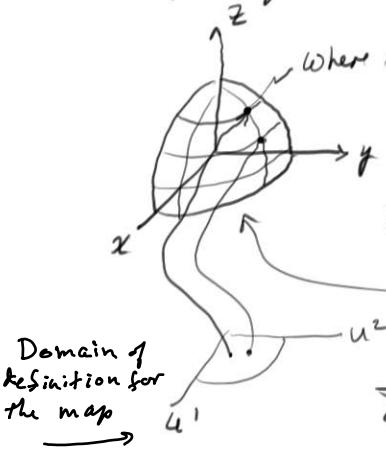
\includegraphics[height=200pt]{Day4NotesPics/sphereMap}
	       
		  This could be expressed as

		$$r^2 = x^2 + y^2 + z^2 \Rightarrow z = \sqrt{r^2 - x^2 - y^2}$$
		$$\Sigma := \begin{cases} 
		  x &= u_1\\
		  y &= u_2\\ 
		z &= \pm\sqrt{r^2 - (u_1)^2 - (u_2)^2}\end{cases}$$

		\item  In general:= Monge Representation
		  $$\Sigma := \begin{cases} 
		    x &= u_1 \\
		    y &= u_2 \\
		  z &= f(u_1, u_2, t)\end{cases}$$
		  \item This representation has useful properties.
		\end{itemize}
	      \end{subsection}

	      \begin{subsection}{Vibrating Bar}
		\begin{itemize}
		\item Imagine a wave running down a sheet. This could also be waves generated on a liquid/vapor interface.

		  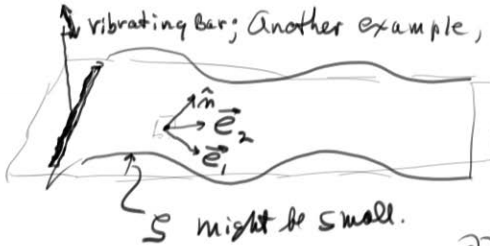
\includegraphics[height=100pt]{Day4NotesPics/vibratingBar}
		\item Assume \begin{align*}
		\Sigma:&=\begin{cases}x&=u_1\\y&=u_2\\z&=\zeta(u_1,u_2,t)\end{cases}\\
		  \d{x}{u_1} &= 1\\ 
		  \d{y}{u_1} &= 0\\
		  \d{\zeta}{u_1} &= \zeta_1\\
		  d\Sigma:&= \begin{pmatrix}1 & 0\\
		  0 & 1\\
		\zeta_1 & \zeta_2\end{pmatrix} \\
		\vec{e}_1 &= \begin{pmatrix}1\\0\\\zeta_1\end{pmatrix}\\
		\vec{e}_2 &= \begin{pmatrix}0\\1\\\zeta_2\end{pmatrix}\\
		  \vec{n} &= \vec{e_1}\times\vec{e_2} = |\vec{e}_1| |\vec{e}_2| sin{\theta_{12}\hat{e_3}}\\
		  \end{align*}
	      \item This example will become a flat, plane-like interface when $\zeta(u_1,u_2, t)=0$
		\item Compute \begin{align*}\vec{e_1} \times\vec{e_2} &= \begin{bmatrix}\hat{i} & \hat{j} & \hat{k}\\
		  1 & 0 & \zeta_1\\
		0 & 1 & \zeta_2\end{bmatrix}\\
		  \vec{n} &= \hat{i}(-\zeta_1) - \hat{j}(\zeta_2) + \hat{k}\\
		\vec{n} &= \begin{pmatrix}-\zeta_1 \\ -\zeta_2 \\ 1\end{pmatrix}\\
		\end{align*}
	      \item Note if $\zeta_1 = \zeta_2 = 0$ the $\vec{n} = (0,0,1)$ along the $\hat{k}$ axis.
	      \item This construction provides a vector defining the local normal; viz.
		
		$\vec{n}\cdot\vec{e}_1 = \vec{n}\cdot\vec{e}_2 = 0$, however $\vec{n}\cdot\vec{n} \neq 1$ generally.

	      \item Suppose you compute $\vec{n}\cdot\vec{n} = 1 + (\zeta_1)^2 + (\zeta_2)^2$ so that
		$\hat{n} = \frac{\vec{n}}{\sqrt{1 + (\zeta_1)^2 + (\zeta_2)^2}}$
		\newcommand{\nhat}[0]{\hat{n}}
		$\nhat\cdot\nhat = 1$
		$\nhat\cdot \vec{e_1} = 0, \nhat\cdot \vec{e}_2 = 0$
		$\vec{e_1}\times \vec{e_2}$ think of this as an area. 

		$\therefore \d A \equiv\mathrm{differential\ area}\equiv \sqrt{1+(\zeta_1)^2 + (\zeta_2)^2} \d u_1 \d u_2$
	      \item Note: When $\zeta_1 = 0, \zeta_2 = 0$, then $\d A = \d u_1 \d u_2$ as expected.



		   \end{itemize}

	      \end{subsection}
      \end{section}


      \begin{section}{Metric Tensor}
	\begin{itemize}
	  \item  $\vec{e}_1 \cdot \vec{e}_1 = 1 + (\zeta_1)^2$ 
	  \item  $\vec{e}_2\cdot \vec{e}_2 = 1 + (\zeta_2)^2$
	  \item $\vec{e}_1 \cdot \vec{e}_2 = \vec{e}_2 \cdot \vec{e}_1 = \zeta_1\zeta_2$
	  \item $\begin{pmatrix}1 + (\zeta_1)^2 & \zeta_1\zeta_2\\
	  \zeta_1\zeta_2 & 1 + (\zeta_2)^2\end{pmatrix} \equiv \matr{a}$

	  \item $\matr{a}$ is the \underline{metric} tensor for $\Sigma$
	  \item Very important. This is the \underline{Metric}
	  \item $\d\zeta^2 = a_{\alpha\beta} \d u_\alpha \d u_\beta \alpha,\beta = 1,2$
	    $\d\zeta$ is a distance along the surface.

	  \item $\det{\matr{a}}= 1 + (\zeta_1)^2 + (\zeta_2)^2$ 
	  \item Note: $\d A = \sqrt{1 + (\zeta_1)^2 + (\zeta_2)^2} \d u_1 \d u_2 = \sqrt{a} \d u_1 \d u_2$ [this is the area for integrating over the surface.]

		\item How much work to create this surface? \begin{align*}R = \int_{A_0} \left[ P\right]_n \zeta(u_1,u_2,t) \sqrt{a}\d u_1 \d u_2 + \int_{A0} \gamma\sqrt{a} \d u_1 \d u_2 \end{align*}
	  \item Minimization of the work with respect to $\zeta$ yields the Laplace equation, which looks like this.

	    $[P]_n = 2\gamma R_{\mathrm{mean}}$
	    Where $R_{\mathrm{mean}} = \frac{1}{2}\left(\frac{1}{R_1} + \frac{1}{R_2}\right)$ [the mean radius of curvature.]
	\end{itemize}
      \end{section}
\end{document}
